\chapter{Background \& Methods}

The following chapter will give an introduction to some theoretical concepts related to the scope of this project. Also, a brief description of the libraries and tools used.

First, we will briefly describe the Decidim process and the components of its dataset used in this study. Later, the text transformation performed over the proposals text to obtain a cleaner data. Then, an explanation of the three different text representation implemented in this project. Next, a description of the clustering algorithm used and its variants. After, a definition of the similarity measures that were used to compute the similarity between documents. Finally, the metrics used to measure the quality of the final clustering.

\section{Dedicim Barcelona}
Decidim Barcelona aim to define The Municipal Plan with the active participation of government and citizens of the city. This plan will guide the actions to be developed during the four years the government last. The plan is composed by a set of proposed improvement to be carried out in the city, these proposals are divided into five categories: Plural Economy, Good Governance, Good Living, Ecological Transition and Global Justice. 

The process to draw The Municipal Plan starts with an initial set of proposals created by The Barcelona City Council. Then, new proposals are created by citizens either face to face or in a through the decidim website, these proposals along with the initial set are discussed, commented and supported. Later, the City Council study all the proposals, new proposals that count with a high level of support are added to the plan of the municipality, and similar proposals are grouped to draw up the final set of proposals that represents a collaborative version of the Municipal Plan. Finally, this version will be evaluated by the plenary of the Municipal Council which will approved proposals, The approved similar proposals are grouped into actuations (also named results indistinctly). The aim of this project is to automatically group similar proposals.

For this study, we will mainly use the text that correspond to the title, description, category and subcategory of each proposal. Results are used to know what would be a correct clustering output, each result has and Id and a list of proposals Ids, the result Id is used as the ground truth for its list of proposals.

\section{Data Preprocessing and Translation}
The original data was a mixture of Catalan and Spanish proposals and actuations. 

Firstly, the text corresponding to the title and description of each proposa that was originally in either, Catalan or Spanish, was translated using Google Cloud Translate API \footnote{\url{https://cloud.google.com/translate/}}, all proposals were translated to English using the auto detection source language of the API.

Secondly, stop words along with punctuation marks were removed to reduce noise and to avoid dealing with words that would not contribute to identifying similarity between words, moreover, words that appear only once in a proposal were also removed, this process was done using python NLTK implementation. 

Lastly, to normalize words representation, words were stemmed in order to obtain their base form, the stemming algorithm used was Porter's Stemmer from NLTK package. 

\section{Data Representation}
Documents need to be represented in such a way that serves as an input to the target algorithm reflecting the document's content in a way that similar pair of documents can be identified. In this project we will focus on three representations, one simple model that works best to identify word overlapping, but that serve as input to the second method that is able to capture semantic similarity from a very simple structure, ultimately, a representation that has shown to capture semantic similarity successfully but that requires big corpus to achieve its best result.

The two most common and simple ways to represent a document is by building a Bag of Words (BOW)\cite{vector.space} or by their term frequency-inverse document frequency (TF-IDF) \cite{tfidf}, both representations do not capture semantic information from documents. Latent Semantic Analysis (LSA) \cite{lsa} tries to overcome this loss of information using singular value decomposition over the BOW or TF-IDF representation to arrive at a semantic feature space, where words with similar meanings are located close to each other, similarly,  Word2Vec \cite{mikolov2013} capture semantical meaning from text, assuming that words with similar context might have similar meanings. Word2Vec produces word embedding that beats any previous model \cite{mikolov2013}\cite{wmd}, however, unlike LSA, requires a corpus over the billions to achieve good results, and its quality is tied to the size of the dataset.


\subsection{TF-IDF}
Term frequency-inverse document frequency (TF-IDF) is a method that reflects the importance of a term to a document in a collection of documents. Term frequency (TF) assigns a weight to each term in a document equals to the number of times that a term $t$ appears in document $d$. A drawback of TF is that considers all terms equally important, a term like \textit{"the"} will occur in almost all document and, TF will assign a high weight. However, a term that occurs very often is usually not descriptive for a document \cite{manning2008introduction}. Inverse document frequency (IDF) correct this penalizing those terms that occur too often across all documents of a collection.

TF-IDF built a $M\times N$ term-document matrix with the resulting TF-IDF value for all $N$ terms in a collection of $M$ documents. This result in a sparse matrix that can be used to compute similarity measures between each document.

Formally, term frequency-inverse document frequency of a term $t$ in a document $d$ is given by:
$$tfidf_{t,d}=tf_{t,d} \cdot idf_{t,D},$$ 
where $tf_{t,d}$ is the number of occurrences of the term $t$ in document $d$ and, $idf_{t,D}$ is the inverse document frequency. The value of $tfidf_{t,d}$ will be low when a term occurs in many documents or occurs a few times in a document, it will decrease when the quantity of documents it appears increase. When a term appears in several documents $tfidf_{t,d}$ will have a high value\cite{manning2008introduction}.

Inverse document frequency $idf_{t}$ of a term $t$ in a collection $D$ is given by:
$$idf_{t,D} = \log{\frac{N}{df_{t,D}}},$$
where $N$ is the number of documents in a collection, and $df_{t,D}$ is the number of documents in a collection $D$ that contain term $t$.

This algorithm has many limitations. It cannot identify whether a word is present with small changes, if the word \textit{play} and \textit{playing} are present, they would have different entries in the resulting vector. TF-IDF is not able to capture the semantic relation of words, it relies on words overlapping to find similarities. Moreover, Tf-Idf outputs a very sparsely matrix, what produce documents vectors of a very high dimensionality. We will address this using a dimensionality reduction technique named LSA.

In this project, the term-document matrix was built for the collection of proposals, where each proposal was the text of its title concatenated with its description. Python library scikit-learn \cite{scikit-learn} was used for this propose.  

\subsection{Latent Semantic Analysis}
Latent Semantic Analysis (LSA) is a method for dimensionality reduction that takes as input the term-document matrix built using TF-IDF \cite{lsa}. LSA finds a projection with the maximal variance of data along axes. The idea behind LSA is that terms that appear together in a collection of documents will have a similar projection on the new vector space. Documents that were not similar by TF-IDF might be similar in a LSA representation. LSA and Principal Component Analysis (PCA) are both methods for dimensionality reduction. Their differ in that PCA uses SVD over a covariance matrix, while LSA uses SVD over a term-frequency matrix.

LSA uses Singular Value Decomposition (SVD) to decompose a term-document matrix $M$ into three matrices $M = U \Sigma_k V^\top$, where $U$ and $V$ are column-orthogonal matrices and $\Sigma_k$ is a diagonal $k \times k$ matrix that contains $k$ singular values of $M$, such that the singular values are in descending order. Finally, a $k' \ll k$ is chosen to obtain a reconstructed $M'$ matrix from multiplying $U \Sigma_k' V ^T $ \cite{clust.short.text}. 

The implementation of LSA over the set of documents (proposals) of decidim.barcelona was carried out using Python library scikit-learn \cite{scikit-learn}. Then, cosine distance was used to build a distance matrix that served as input to the hierarchical clustering process.
\subsection{Word2Vec}
Word2Vec is an extensively used word embedding algorithm that convert words into vectors that capture semantical meaning \cite{semantic.short}. 
Two neural network models (Continuous Bag of Words (CBOW) and Skip-gram) that outperformed all previous architecture were introduced in \cite{mikolov2013}.
The main assumption of these models is that words with similar context have a similar meaning. Word2Vec defines a window of size $k$, also called context, and scans the corpus training the model for each word keeping $k$ words around the target word. CBOW and Skip-gram differ in how this context is used.

CBOW predicts $w_i$ given the window of surrounding words. It is composed of three layers (see Figure~\ref{fig:word2vec}): the input layer corresponds to the context of the target word, the hidden layer projects each word from the input layer into the weight matrix, this matrix has one row for every word in the vocabulary of the training corpus and as much columns as features (300 features for the model used in this study). Finally, the third layer is the output layer, that for this model will output the target word for the given context.

Skip-gram predicts the surrounding words given the center word $w_i$. It is also composed of three layers (see Figure~\ref{fig:word2vec}), where the input layer is the target word $w_i$  while the output layer is its context. 

\begin{figure}[h]
\centering
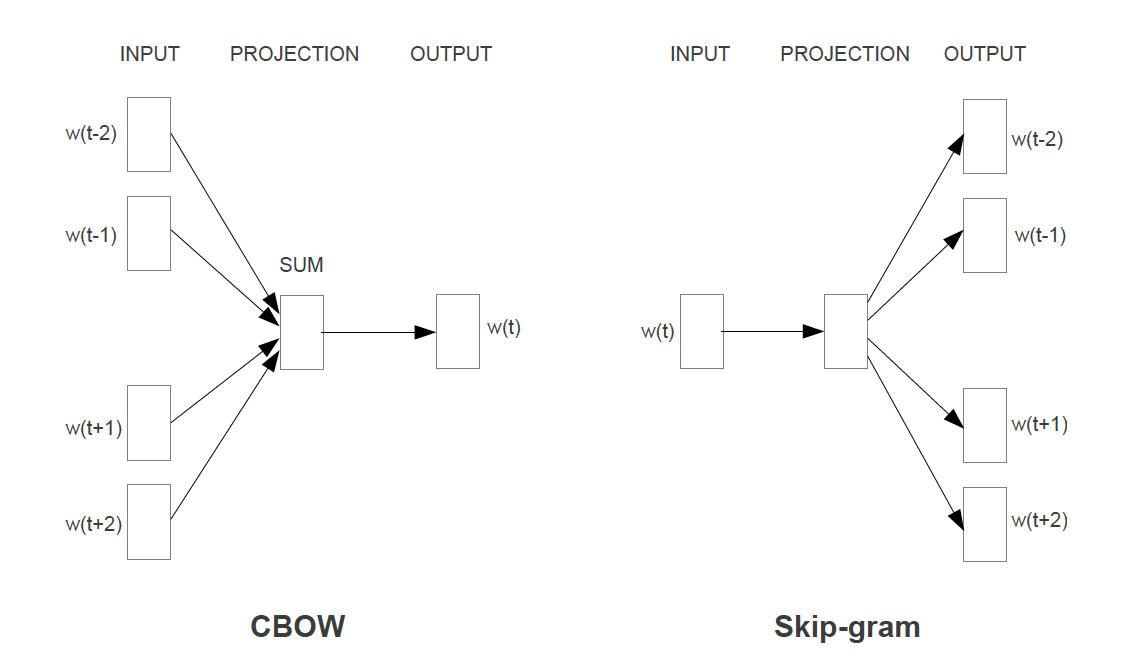
\includegraphics[width=10cm]{Figures/word2vec.png}
\caption{The CBOW model predicts the current word based on the context, and the Skip-gram predicts surrounding words given the current word \cite{mikolov2013}.}
\label{fig:word2vec}
\end{figure}


Word2Vec will produce a vector representation for words present in its training set. To extend this representation to a document or sentence scope one can take the element-wise sum or mean of the word embeddings across all the words in the document, this will produce a vector that will encode the semantical meaning of the document. This approach has been used successfully in \cite{mikolov.phrases} \cite{sumarization}.

Word2Vec typically requires a large training dataset to achieve good results (over billion words in\cite{mikolov2013}). Since the dataset for this project is too limited in that sense, we used a pre-trained word2vec model \cite{word2vec.lexical} \cite{wmd}.

In this project, we used the pre-trained model from Google, which has 300 feature word vectors for 3 million words and it was trained on 100 billion words Google News dataset \footnote{\url{https://code.google.com/archive/p/word2vec/}}.

\section{Clustering Algorithm}
Clustering is a form of unsupervised learning that divides a dataset into different groups or clusters.
It aims to build a distinct cluster where members of each cluster are similar between them and consequently, members of distinct clusters are different.
Clustering algorithms don't have labeled categories where to fit the data, as classification algorithms which are a form of supervised learning.
A key input in any clustering algorithm is the distance measure selection. This measure will determine which element belongs to each cluster, different distance measures will produce different clusters\cite{manning2008introduction}.

There are two main categories of clustering methods: partitional clustering and hierarchical clustering, the last was the one chosen for the propose of this study.

\subsection{Hierarchical Clustering}
Hierarchical clustering builds a tree-like hierarchical structure called dendrogram (see Figure~\ref{fig:dendrogram}) that offers a visualization of the obtain clustering at different scales.

\begin{figure}[h]
\centering
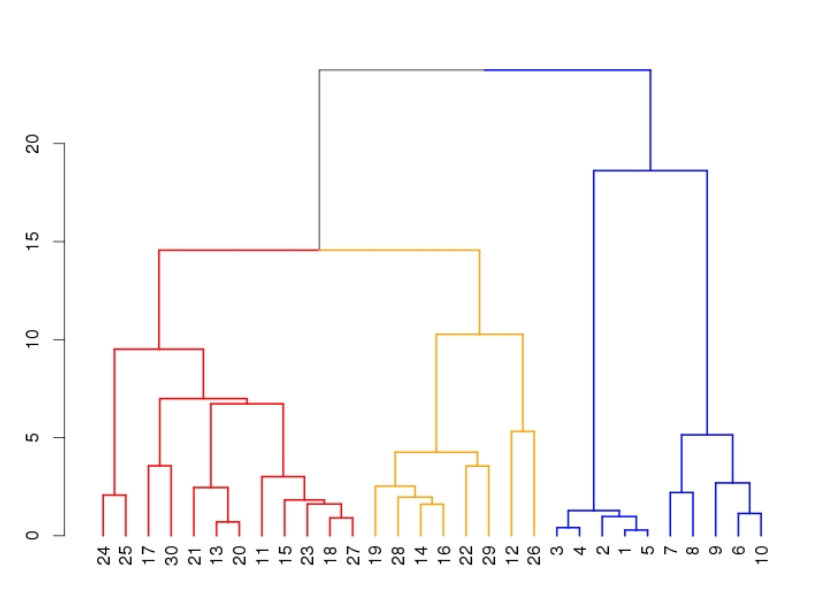
\includegraphics[width=8cm]{Figures/dendrogram.png}
\caption{Example of a dendrogram}
\label{fig:dendrogram}
\end{figure}

Hierarchical clustering algorithms can be split into two categories: Agglomerative, where all leaves start being a cluster and they are merged from bottom to top, and divisive, where all leaves belong to a single cluster, and the clustering is created splitting recursively from top to bottom\cite{clusteringSurvey}. In this project, we will focus on agglomerative hierarchical clustering, where leaves represent proposal.

Agglomerative clustering on decidim's proposals initiate merging the two closest single proposals forming a new node that contains two proposals, this node is then merged to its closest single proposal or node, this process is repeated across all single proposals and nodes until there is one single node that contains all previously created nodes \cite{mullner}. 
In agglomerative clustering, the fundamental step is the selection of two clusters that are merged to create a new cluster.

There are different methods to compute the similarity or distance between nodes; called linkage. These methods depend on a similarity measure \ref{sec:similarities}, by default in Python Scipy library \cite{scipy} $dist$ is defined as the Euclidean distance \ref{sec:euclidean}. Below are the linkage methods used in this study: 
\begin{itemize}[label=]
    \item \textbf{Complete:} The similarity of two clusters $u$ and $v$ is defined as the similarity of the two most dissimilar members of each cluster\cite{mullner}.
    $$d(u,v) = \max(dist(u[i], v[j])),$$ for all members $i$ in cluster $v$ and $j$ in cluster $u$.
    \item \textbf{Average:} The similarity of two clusters is defined as the average similarity between all pairs of members \cite{mullner}.
    $$d(u,v) = \sum_{i,j}\frac{dist(u[i], v[j])}{|u|\cdot|v|},$$
    for all members $i$ in cluster $v$ with cardinality $|v|$ and points $j$ in cluster $u$ with cardinality $|u|$.
    \item \textbf{Weighted:} The similarity of two clusters is defined as the average of the similarity between all pairs of members from different clusters and it is weighted based on the quantity of members in each cluster\cite{mullner}.
    $$d(u,v) = \frac{dist(s,v) + dist(t,v)}{2},$$
where $u$ is a cluster formed with cluster $s$ and $t$, and $v$ is a remaining cluster.

%     \item \textbf{Centroid:} The similarity of two clusters is defined as the similarity of the centroids of each cluster \cite{mullner} (The centroid of a cluster is the mean of all its data points).
%     $$d(u,v) = \| c_u - c_v\|,$$
%     where $c_u$ is the centroid of cluster $u$ and $c_v$ is the centroid of cluster 

$v$.\end{itemize}

The hierarchical clustering algorithm does not require a pre-defined number of clusters. Instead, the obtained dendrogram can be used to analyze and decide at which height the tree should be cut to generate the final clustering. In Figure~\ref{fig:dendrogram} the $x$ axis represents the data points and the $y$ axis the distance at which each node was merged. The cutting threshold can be decided visually, or alternatively using a measure computed from the clustering at each level, such as silhouette coefficient \cite{han2012mining}. 

\section{Similarity Measures}
\label{sec:similarities}

Document clustering group a collection of documents into clusters, ideally placing similar documents in the same cluster, and different documents far apart in a different cluster. The goal of clustering is to achieve high intra-clustering similarity, documents in the same cluster are similar; and low inter-cluster similarity, documents from different cluster are dissimilar\cite{manning2008introduction}. An appropriate definition of documents similarity or distance depends on the problem properties\cite{similarity.mes}. Different measures would lead to completely different clustering. In this project, we focus on two: Euclidean Distance and Cosine Similarity.

\subsection{Euclidean Distance}
\label{sec:euclidean}

Euclidean distance is widely used to determine the level of similarity between vectors, specially in the case of clustering. It is the  length of a straight line between two points, by default multiple clustering algorithms use this distance measure. Given two documents $d_a$ and $d_b$, represented by vectors $\vec{V_a}$ and $\vec{V_b}$, their euclidean distance is defined as \cite{similarity.mes}:
$$D_E(\vec{V_a},\vec{V_b})=(|V_a - V_b|^2)^{1/2}$$
\subsection{Cosine Similarity}
Cosine similarity is one of the most used measures to determine documents similarity. It measures the angle between the vector representation of two documents. Given two documents $d_a$ and $d_b$, represented by vectors $\vec{V_a}$ and $\vec{V_b}$, their cosine similarity is defined as \cite{similarity.mes}:
$$SIM_C(\vec{V_a},\vec{V_b})= \cos({\vec{V_a},\vec{V_b}}) = \frac{\vec{V_a}.\vec{V_b}}{|\vec{V_a}|\cdot |\vec{V_b}|}$$

The cosine distance will be used as a metric to compute the distance between documents, it is defined as:
$$ D_C(\vec{V_a},\vec{V_b}) = 1 - SIM_C(\vec{V_a},\vec{V_b})$$
\section{Cluster Evaluation}
Evaluate the quality of a clustering solution is a critical and difficult task. Decide the goodness of clusters is a key step to choose a solution that will group the data successfully. Cluster quality measures can be categorized into two classes, external criterion of quality and internal criterion of quality \cite{manning2008introduction}. They difference is that once required external information; a ground truth, and the other only rely on the data itself. 

For the propose of this study we decided to use silhouette coefficient; an internal criterion, and purity and normalized mutual information; both external criterion. One of the main challenges we had was the absence of an accurate ground truth, we had the results (actuations) which group multiple proposals in a single result which tackle similar problems. However, this grouping is far from being accurate, similar proposals are not in an unique group, and also group not related proposals into the same result. However, as this was the closest we had to the expected output, we used it along with an internal measure.
 

\subsection{Silhouette Coefficient}
When the ground truth is not available, we have to use an internal criterion to know the clustering quality. Internal criterion evaluates clustering by examining how compact each cluster is, and how separated different clusters are from each one\cite{han2012mining}.

To measure the silhouette coefficient for a document $d \in D$ we need to measure the minimum average distance from $d$ to all different clusters to which $d$ does not belong to and, the average distance between $d$ and all other documents in the same cluster where $d$ belongs to. \cite{han2012mining}.

The Silhouette coefficient for a document $d$ in a dataset $D$ of $n$ documents partitioned into $k$ clusters $\{w_1,...,w_k\}$  is defines by,

\begin{equation}
silhouette(d) = \frac{b(d) - a(d)}{\max{\{a(d), b(d)\}}},
\label{eq:sil}
\end{equation}

where:
\begin{equation}
b(d) = min_{w_{j:1\leq j \leq k, j\neq i}}{\left \{ \frac{\sum_{d'\in w_j} dist(d, d')}{|w_j|} \right \}},
\label{eq:bd}
\end{equation}

and,
\begin{equation}
a(d) = \frac{\sum_{d' \in w_i, d\neq d'} dist(d,d')}{|w_i|-1  }
\label{eq:ad}
\end{equation}

The value of the silhouette coefficient (\ref{eq:sil}) goes from -1 to 1. The value of $a(d)$ (\ref{eq:ad}) represents the compactness of the cluster, a small $a(d)$ represent a compact cluster. While the value of $b(d)$ (\ref{eq:bd}) capture how separated a document $d$ is to another clusters, the larger is $b(d)$ the more distant $d$ is to another clusters. A silhouette coefficient close to 1 means that the cluster containing $d$ is compact and $d$ is far from other clusters. When the silhouette coefficient  is negative ($b(d) < a(d)$) means that $d$ is closer to a documents in a different cluster than to documents in the same cluster. The desired result is a silhouette coefficient close to 1 \cite{han2012mining}.

To measure the cluster quality, first, the silhouette coefficient is computed for all documents in the dataset. Then, the silhouette coefficient of a clustering result is the average of the silhouette coefficient of all documents in the dataset. 
\subsection{Purity}
The purity is a simple external criterion that rely on the ground truth to measure the goodness of the clustering result. The purity measure if a cluster contains documents of a single class, the majority of documents determine the correct class of a cluster. The purity is defined by:
$$purity(\Omega, C) = \frac{1}{N}\sum_k\max_j |w_k \cap c_j|$$,
where $\omega = \{w_1, ..., w_k\}$  is the set of resulting cluster and  $C = {c_1,..., c_j}$ is the set of classes \cite{manning2008introduction}. 

The purity value goes from 0 to 1. A bad clustering according to the ground truth would have a value near to 0, while a good clustering would have a purity near to 1 \cite{manning2008introduction}. However, good purity is easy to achieve when the number of clusters is large, for example if each cluster has only one element the purity would be 1. For this reason, purity by itself is not a fair measure of the quality of a cluster, but it can give some idea of the quality of a solution when used along other metrics.

\subsection{Normalized Mutual Information}
Normalized Mutual Information (NMI) is an external criterion that has it origin in Information Theory and is based in the concept of entropy. The Entropy of $k$ clusters in $\Omega$ is defined by \cite{manning2008introduction}:

$$H(\Omega) = -\sum_k P(w_k)log(P(w_k)),$$

where $P(w_k)$ is the probability of a document of belonging to cluster $w_k$.

The entropy of a cluster $\Omega$ measure the level of uncertainty that can be reduced when a random document $w$ is taken from $\Omega$. 
The concept of entropy can be extended to Mutual Information, which measures how much information can be gained from the actual class of an element when its cluster is known. Mutual Information is defined by \cite{manning2008introduction}:

$$I(\Omega, C) = \sum_k\sum_j P(w_k \cap c_j) log\frac{P(w_k \cap c_j)}{P(w_k) P(c_j)},$$
where $P(w_k), P(c_j),$ and $P(w_k \cap c_j)$ are the probabilities of a document belonging to cluster $w_k$, class $c_j$ and to the intersection of $w_k$ and $c_j$. The value of $I(\Omega, C)$ is 0 if knowing the cluster of a document give no information about its actual class. The highest values for $I(\Omega, C)$ is 1, that is the case when $\Omega$ define a perfect cluster, that match the ground truth, but, a maximum mutual information can be achieved when the number of clusters is equal to the number of documents. Mutual information presents the same problem that purity. Normalized mutual information penalize high cardinalities, and is defined by \cite{manning2008introduction}:

$$NMI(\Omega, C) = \frac{I(\Omega, C)}{[H(\Omega) + H(C)]/2},$$

However, this penalty does not avoid NMI to favor clustering with a high number of clusters \cite{nmi.fair}.

\subsection{Adjusted Rand Index}

Adjusted Rand Index (ARI) is another external criterion that measures the congruence between a clustering result and a ground truth. ARI is an improvement to Rand Index, which lead to high values even when there is a high level of disagreement between clusters and actual classes \cite{comparing.partitions}. ARI is defined by:

$$\frac{\sum_{i,j}{n_{i,j}\choose 2} - \left[ \sum_i {n_{i}\choose 2} \sum_j {n_{j}\choose 2} \right] / {S\choose 2}}{1/2 \left[ \sum_i {n_{i}\choose 2} + \sum_j {n_{j}\choose 2} \right] - \left[ \sum_i {n_{i}\choose 2}\sum_j {n_{j}\choose 2} \right] / {S\choose 2}},$$

where $n_{i,j}$ is the number of document of class $c_i$ present in a cluster $w_j$, $n_i$ is the number of documents in class $c_i$ and, $n_j$ is the number of document in the cluster $w_j$.ARI values go from -1 to 1, being 1 the best score and -1 being worst than a random result \cite{clust.short.text}.

\newpage
